\documentclass[border=5pt]{standalone}
\usepackage{tikz}
\usetikzlibrary{patterns, arrows.meta, positioning, calc, decorations.pathreplacing}

% Color definitions
\definecolor{patchA}{RGB}{74,144,217}
\definecolor{patchB}{RGB}{232,168,56}
\definecolor{kept}{RGB}{46,139,87}
\definecolor{cropred}{RGB}{226,85,85}
\definecolor{patchC}{RGB}{91,174,91}
\definecolor{patchD}{RGB}{199,90,155}

\begin{document}
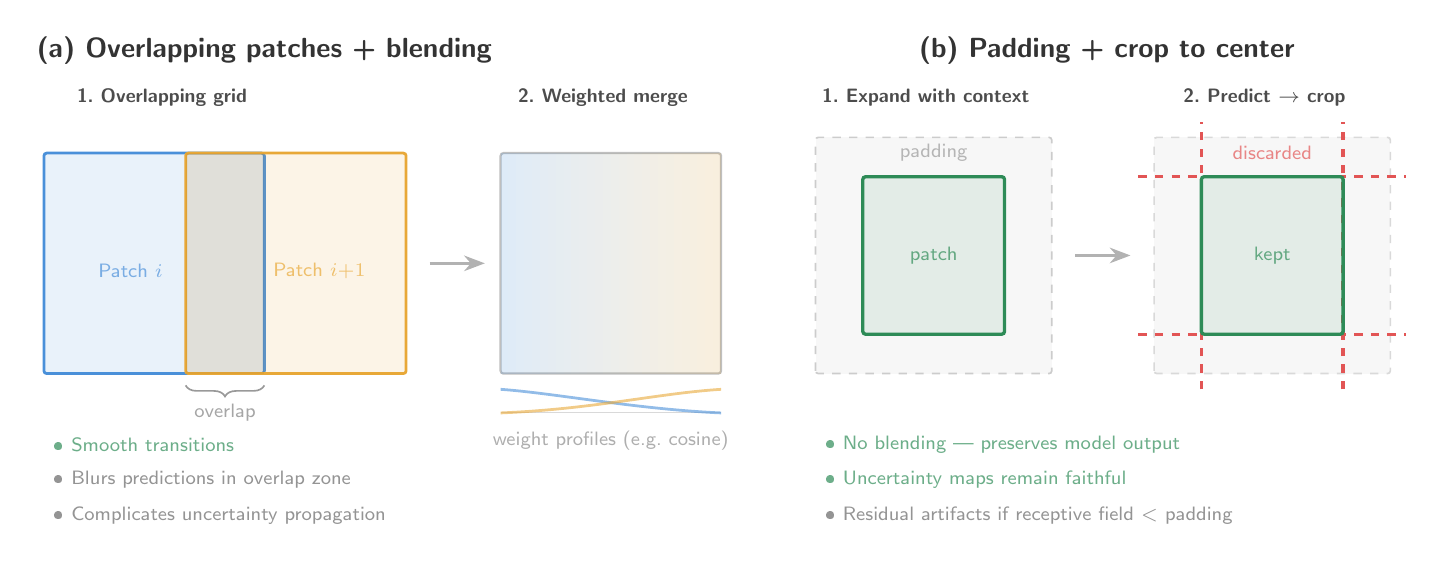
\begin{tikzpicture}[
    >=Stealth,
    every node/.style={font=\sffamily\small},
    patch/.style={rounded corners=1pt, line width=1pt},
    annot/.style={font=\sffamily\scriptsize, text opacity=0.7},
    heading/.style={font=\sffamily\small\bfseries, text opacity=0.8},
]

% ============================================================
% PANEL (a): Overlapping patches + weighted blending
% ============================================================
\node[heading, font=\sffamily\bfseries] at (2.8, 5.8) {(a) Overlapping patches + blending};
% --- Step 1: Overlapping patches ---
\node[annot, font=\sffamily\scriptsize\bfseries] at (1.5, 5.2) {1.\ Overlapping grid};
% Patch i
\fill[patchA, opacity=0.12] (0, 1.7) rectangle (2.8, 4.5);
\draw[patchA, patch] (0, 1.7) rectangle (2.8, 4.5);
\node[annot, patchA] at (1.1, 3.0) {Patch $i$};
% Patch i+1 (overlapping)
\fill[patchB, opacity=0.12] (1.8, 1.7) rectangle (4.6, 4.5);
\draw[patchB, patch] (1.8, 1.7) rectangle (4.6, 4.5);
\node[annot, patchB] at (3.5, 3.0) {Patch $i{+}1$};
% Overlap zone shading
\fill[black, opacity=0.04] (1.8, 1.7) rectangle (2.8, 4.5);
% Overlap brace
\draw[decorate, decoration={brace, amplitude=4pt, mirror}, black!40, line width=0.6pt]
    (1.8, 1.55) -- (2.8, 1.55);
\node[annot, black!50] at (2.3, 1.2) {overlap};
% Arrow to step 2
\draw[->, black!30, line width=1pt] (4.9, 3.1) -- (5.6, 3.1);
% --- Step 2: Weighted blending ---
\node[annot, font=\sffamily\scriptsize\bfseries] at (7.1, 5.2) {2.\ Weighted merge};
% Blended result box
\draw[black!25, line width=0.8pt, rounded corners=1pt] (5.8, 1.7) rectangle (8.6, 4.5);
% Gradient fill (approximate with rectangles)
\foreach \i in {0,...,27} {
    \pgfmathsetmacro{\x}{5.8 + \i * 0.1}
    \pgfmathsetmacro{\opA}{max(0, 0.18 - \i * 0.006)}
    \pgfmathsetmacro{\opB}{max(0, \i * 0.006 - 0.0)}
    \fill[patchA, opacity=\opA] (\x, 1.7) rectangle (\x+0.1, 4.5);
    \fill[patchB, opacity=\opB] (\x, 1.7) rectangle (\x+0.1, 4.5);
}
% Weight profile lines below
\draw[black!15, line width=0.4pt] (5.8, 1.2) -- (8.6, 1.2);
% Weight curve patch i (decreasing)
\draw[patchA, opacity=0.6, line width=1pt]
    (5.8, 1.5) .. controls (6.5, 1.45) and (7.5, 1.25) .. (8.6, 1.2);
% Weight curve patch i+1 (increasing)
\draw[patchB, opacity=0.6, line width=1pt]
    (5.8, 1.2) .. controls (7.0, 1.25) and (7.8, 1.45) .. (8.6, 1.5);
\node[annot, black!45] at (7.2, 0.85) {weight profiles (e.g.\ cosine)};


% Pros/cons for panel (a)
\node[annot, anchor=west, kept] at (0, 0.8) {\textbullet\ Smooth transitions};
\node[annot, anchor=west, black!60] at (0, 0.35) {\textbullet\ Blurs predictions in overlap zone};
\node[annot, anchor=west, black!60] at (0, -0.1) {\textbullet\ Complicates uncertainty propagation};


% ============================================================
% PANEL (b): Padding + crop to center
% ============================================================
\node[heading, font=\sffamily\bfseries] at (13.5, 5.8) {(b) Padding + crop to center};

% --- Step 1: Padded input ---
\node[annot, font=\sffamily\scriptsize\bfseries] at (11.2, 5.2) {1.\ Expand with context};

% Outer padding region
\fill[black, opacity=0.03] (9.8, 1.7) rectangle (12.8, 4.7);
\draw[black!20, line width=0.6pt, dashed, rounded corners=1pt] (9.8, 1.7) rectangle (12.8, 4.7);


% Inner patch (kept region)
\fill[kept, opacity=0.1] (10.4, 2.2) rectangle (12.2, 4.2);
\draw[kept, line width=1.2pt, rounded corners=1pt] (10.4, 2.2) rectangle (12.2, 4.2);

\node[annot, kept] at (11.3, 3.2) {patch};
\node[annot, black!40] at (11.3, 4.5) {padding};

% Arrow to step 2
\draw[->, black!30, line width=1pt] (13.1, 3.2) -- (13.8, 3.2);

% --- Step 2: Predict and crop ---
\node[annot, font=\sffamily\scriptsize\bfseries] at (15.5, 5.2) {2.\ Predict $\rightarrow$ crop};

% Full prediction (faded outer)
\fill[black, opacity=0.03] (14.1, 1.7) rectangle (17.1, 4.7);
\draw[black!15, line width=0.6pt, dashed, rounded corners=1pt] (14.1, 1.7) rectangle (17.1, 4.7);

% Crop lines
\draw[cropred, line width=1.2pt, dashed] (14.7, 1.5) -- (14.7, 4.9);
\draw[cropred, line width=1.2pt, dashed] (16.5, 1.5) -- (16.5, 4.9);
\draw[cropred, line width=1.2pt, dashed] (13.9, 2.2) -- (17.3, 2.2);
\draw[cropred, line width=1.2pt, dashed] (13.9, 4.2) -- (17.3, 4.2);

% Kept center
\fill[kept, opacity=0.1] (14.7, 2.2) rectangle (16.5, 4.2);
\draw[kept, line width=1.2pt, rounded corners=1pt] (14.7, 2.2) rectangle (16.5, 4.2);

\node[annot, kept] at (15.6, 3.2) {kept};
\node[annot, cropred, opacity=0.7] at (15.6, 4.5) {discarded};

% Pros/cons for panel (b)
\node[annot, anchor=west, kept] at (9.8, 0.8) {\textbullet\ No blending --- preserves model output};
\node[annot, anchor=west, kept] at (9.8, 0.35) {\textbullet\ Uncertainty maps remain faithful};
\node[annot, anchor=west, black!60] at (9.8, -0.1) {\textbullet\ Residual artifacts if receptive field $<$ padding};


\end{tikzpicture}
\end{document}